
\begin{figure}
    \centering
    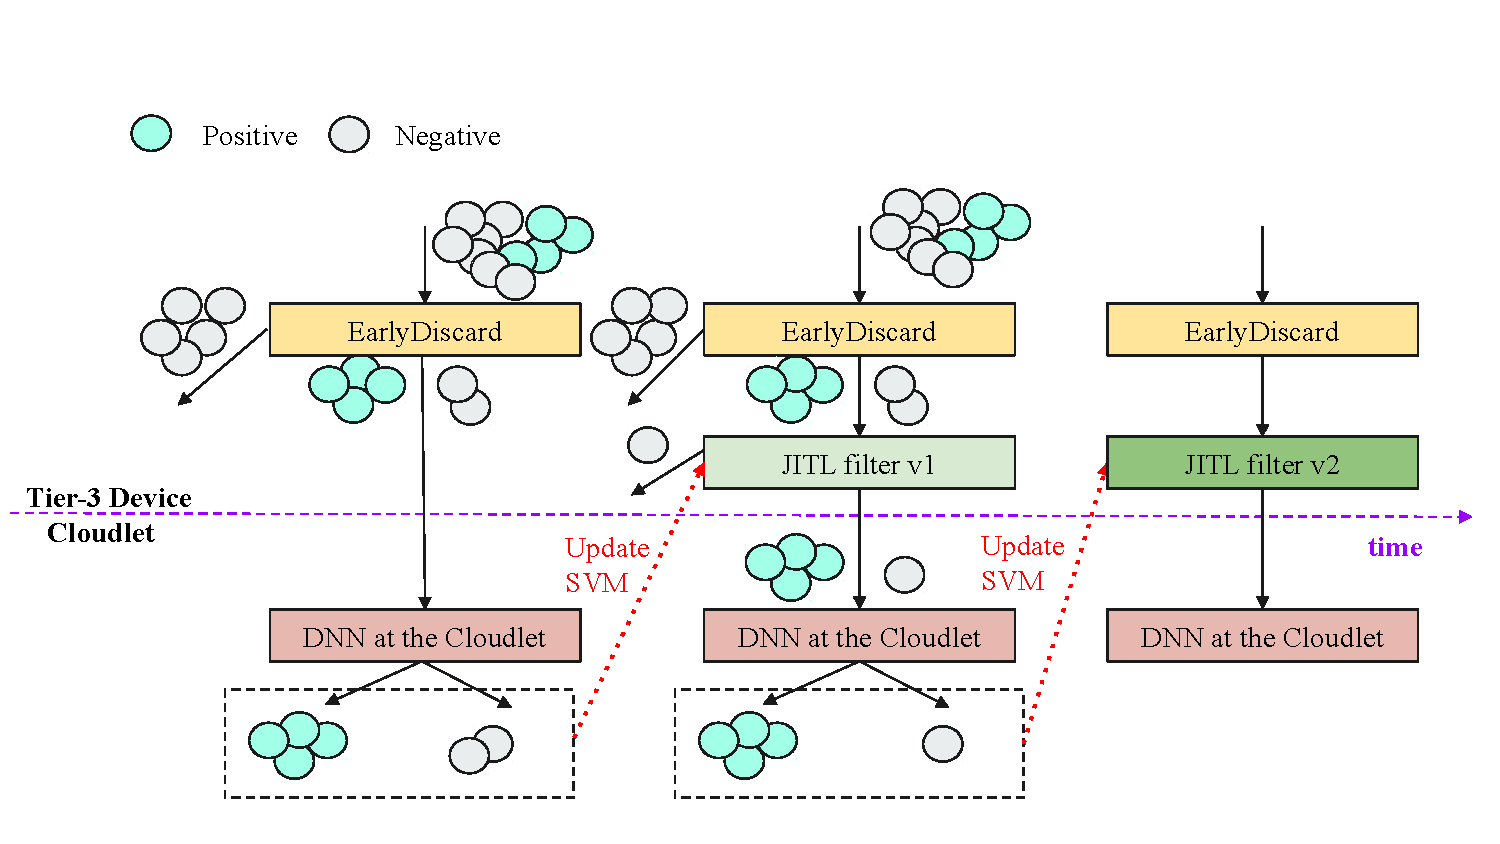
\includegraphics[width=\linewidth]{FIGS/fig-jitl.pdf}
    \caption{JITL Pipeline}
    \label{fig:jitl}
\end{figure}

\section{Just-In-Time-Learning (JITL) Strategy To Improve Early Discard}
\label{sec:jitl}

\begin{figure}
    \centering
    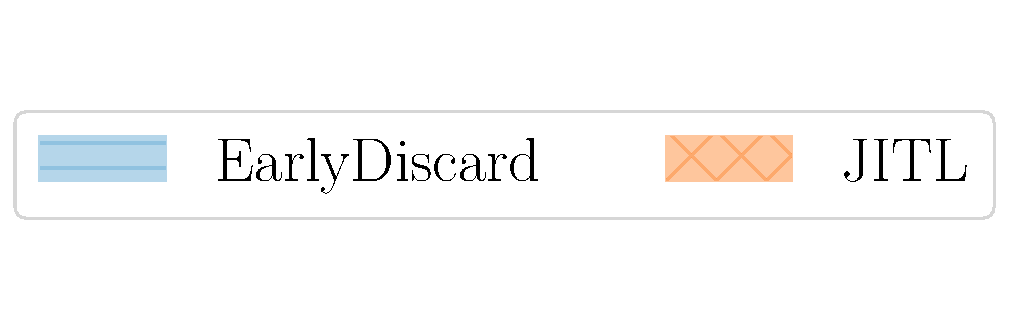
\includegraphics[trim={0 1.8cm 0 0},clip,width=0.7\linewidth]{FIGS/fig-jitl-legend.pdf}\\
    \vspace{.5in}
    \begin{subfigure}[b]{.48\linewidth}
        \centering
        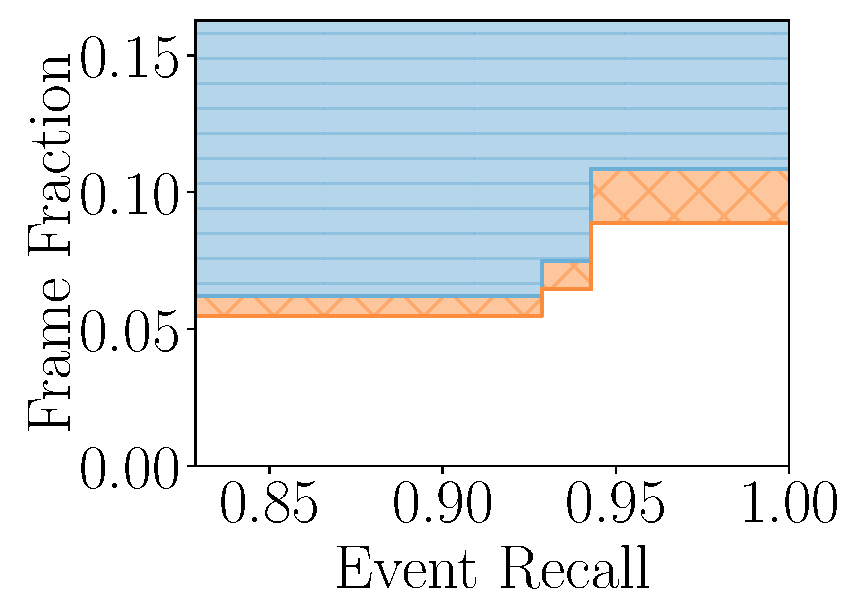
\includegraphics[width=\linewidth]{FIGS/fig-jitl-okutama-eventrecall-step.pdf}
        \caption{T1}
    \end{subfigure}
    \begin{subfigure}[b]{.48\linewidth}
        \centering
        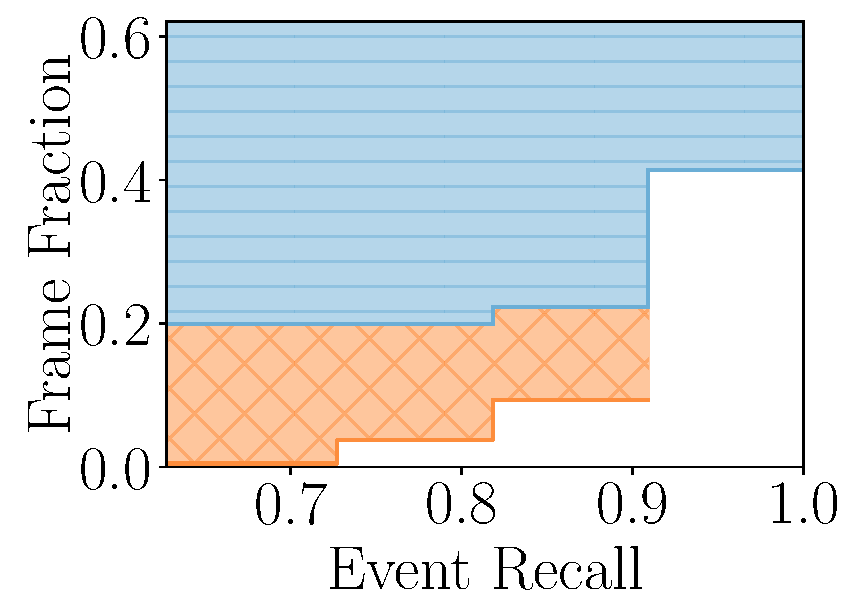
\includegraphics[width=\linewidth]{FIGS/fig-jitl-stanford-eventrecall-step.pdf}
        \caption{T2}
    \end{subfigure}

    \vspace{.5in}

    \begin{subfigure}[b]{.48\linewidth}
        \centering
        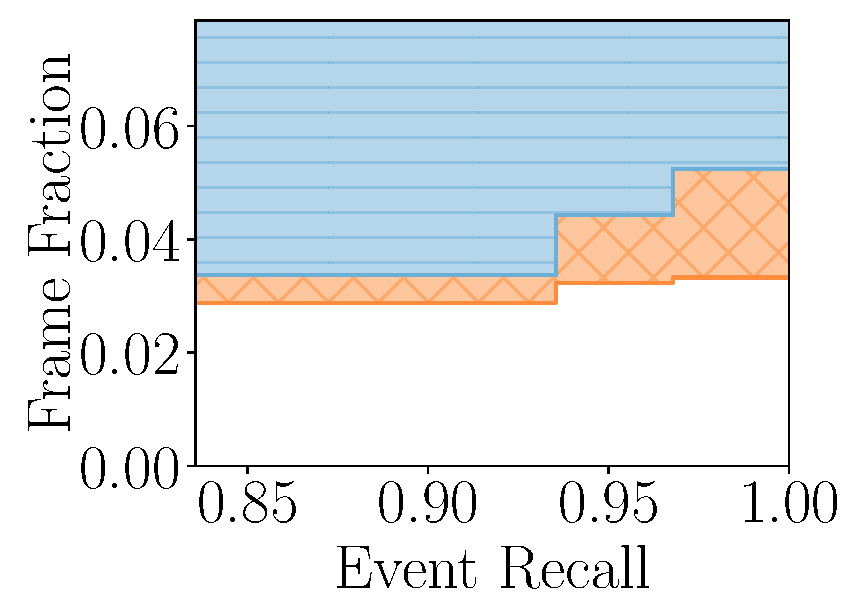
\includegraphics[width=\linewidth]{FIGS/fig-jitl-raft-eventrecall-step.pdf}
        \caption{T3}
    \end{subfigure}
    \begin{subfigure}[b]{.48\linewidth}
        \centering
        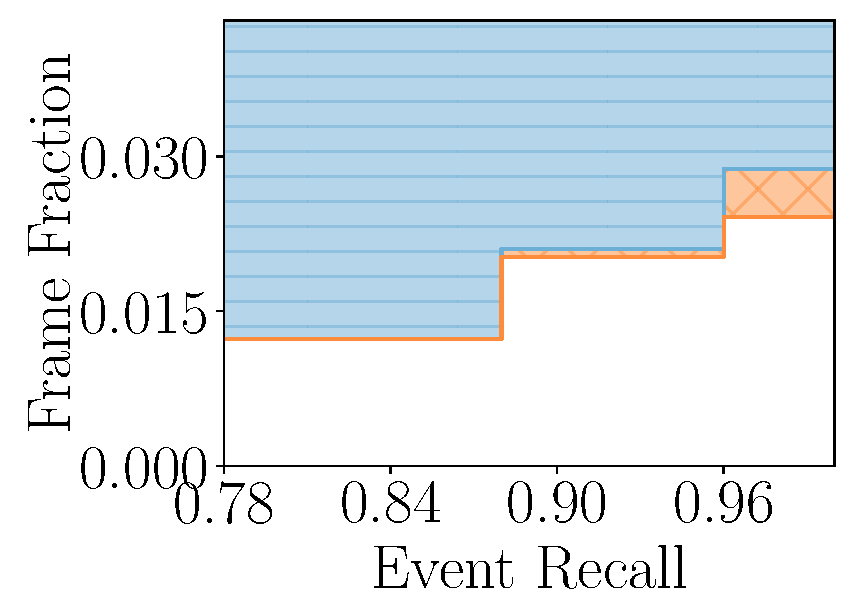
\includegraphics[width=\linewidth]{FIGS/fig-jitl-elephant-eventrecall-step.pdf}
        \caption{T4}
    \end{subfigure}

    \vspace{.5in}
    \caption{JITL Fraction of Frames under Different Event Recall}
    \label{fig:jitl-eventrecall}
\end{figure}

While EarlyDiscard filters are customized and optimized for specific tasks (e.g.
detecting a human with red life jacket), we observe that EarlyDiscard filters do
not leverage context information within a specific video stream. Opportunities
exist if we could further specialize the computer vision processing to the
characteristics of video streams.

We propose Just-in-time-learning  (JITL), which tunes the Tier-3 processing
pipeline to the characteristics of the current task in order to reduce
transmitted false positives from the Tier-3 device, and thereby reducing wasted
bandwidth.  Intuitively, JITL leverages temporal locality in video streams to
quickly adapt processing outcomes based on recent feedback.

It is inspired by the ideas of cascade architecture from the computer vision
community~\cite{Viola2001}, but is different in construction. A JITL filter is a
cheap cascade filter that distinguishes between the EarlyDiscard DNN's
\emph{true positives} (frames that are actually interesting) and \emph{false
    positives} (frames that are wrongly considered interesting). Specifically, when
a frame is reported as positive by EarlyDiscard, it is then passed through a
JITL filter. If the JITL filter reports negative, the frame is regarded as a
false positive and will not be sent. Ideally, all \emph{true positives} from
EarlyDiscard are marked \emph{positive} by the JITL filter, and all \emph{false
    positives} from EarlyDiscard are marked \emph{negative}.  Frames dropped by
EarlyDiscard are not processed by the JITL filter, so this approach can only
serve to improve precision, but not recall.

As shown in Figure~\ref{fig:jitl} during task execution, a JITL filter is
trained on the cloudlet using the frames transmitted from the Tier-3 device.
The frames received on the cloudlet are predicted positive by the EarlyDiscard
filter. The cloudlet, with more processing power, is able to run more accurate
DNNs to identify true positives and false positives. Using this information as a
feedback on how well current Tier-3 processing pipeline is doing, a small and
lightweight JITL filter is trained to distinguish true positives and false
positives of EarlyDiscard filters. These JITL filters are then pushed to the
Tier-3 device to run as a cascade filter after the EarlyDiscard DNN.

True or false positive frames have high temporal locality throughout a task. The
JITL filter is expected to pick up the features that confused the EarlyDiscard
DNN in the immediate past and improve the pipeline's accuracy in the near
future. These features are usually specific to the current task execution, and
may be affected by terrain, shades, object colors, and particular shapes or
background textures.

JITL can be used with EarlyDiscard DNNs of different cutoff probabilities to
strike different trade-offs. In a bandwidth-favored setting, JITL can work with
an aggressively selective EarlyDiscard DNN to further reduce wasted bandwidth. In
a recall-favored setting, JITL can be used with a lower-cutoff DNN to preserve
recall.

In our implementation, we use a linear support vector machine
(SVM)~\cite{Friedman2001} as the JITL filter. Linear SVM has several advantages:
1) short training time in the order of seconds; 2) fast inference; 3) only
requires a few training examples; 3) small in size to transmit, usually on the
order of 50KB in our experiments. The input features to the JITL SVM filter are
the image features extracted by the EarlyDiscard DNN filter. In our case, since
we are using MobileNet as our EarlyDiscard filter, they are the 1024-dimensional
vector elements from the second last layer of MobileNet. This vector, also
called ``bottleneck values'' or ``transfer values'' captures high-level features
that represents the content of an image. Note that the availability of such
image feature vector is not tied to a particular image classification DNN nor
unique to MobileNet. Most image classification DNNs can be used as a feature
extractor in this way.

\subsection{JITL Experimental Setup}

We used Jetson TX2 as our Tier-3 device platform and evaluated the JITL strategy
on four tasks, T1 to T4. For the test videos in each task, we began with the
EarlyDiscard filter alone and gradually trained and deployed JITL filters.
Specifically, every ten seconds, we trained an SVM using the frames transmitted
from the Tier-3 device and the ground-truth labels for these frames. In a real
deployment, the frames would be marked as true positives or false positives by
an accurate DNN running on the cloudlet since ground-truth labels are not
available. In our experiments, we used ground-truth labels to control variables
and remove the effect of imperfect prediction of DNN models running on the
cloudlet.

In addition, we used the true and false positives from all previous intervals,
not just the last ten seconds when training the SVM. The SVM, once trained, is
used as a cascade filter running after the EarlyDiscard filter on the Tier-3
device to predict whether the output of the EarlyDiscard filter is correct or
not. For a frame, if the EarlyDiscard filter predicts it to be interesting, but
the JITL filter predicts the EarlyDiscard filter is wrong, it would not be
transmitted to the cloudlet. In other words, following two criteria need to be
satisfied for a frame to be transmitted to the cloudlet: 1) EarlyDiscard filter
predicts it to be interesting 2) JITL filter predicts the EarlyDiscard filter is
correct on this frame.

\subsection{Evaluation}

From our experiments, JITL is able to filter out more than 15\% of remaining
frames after EarlyDiscard without loss of event recall for three of four tasks.
Figure~\ref{fig:jitl-eventrecall} details the fraction of frames saved by JITL.
The X-axis presents event recall. Y-axis represents the fraction of total
frames. The blue region presents the achievable fraction of frames by
EarlyDiscard. The orange region shows the additional savings using JITL. For T1,
T3, and T4, at the highest event recall, JITL filters out more than 15\% of
remaining frames. This shows that JITL is effective at reducing the false
positives thus improving the precision of the pipeline. However,
occasionally, JITL predicts wrongly and removes true positives. For example, for
T2, JITL does not achieve a perfect event recall. This is due to shorter event
duration in T2, which results in fewer positive training examples to learn
from. Depending on tasks, getting enough positive training examples for JITL
could be difficult, especially when events are short or occurrences are few. To
overcome this problem in practice, techniques such as synthetic data
generation~\cite{dwibedi2017cut} could be explored to synthesize true positives
from the background of the current task.
